\documentclass[11pt,a4paper]{article}
\usepackage[utf8]{inputenc}
\usepackage[T1]{fontenc}
\usepackage{amsmath,amssymb}
\usepackage{booktabs}
\usepackage{graphicx}
\usepackage{geometry}
\geometry{margin=2.5cm}
\usepackage{hyperref}

\title{Accumulation Dark Energy Model: Testing the DESI Anomaly,\\ Perturbation Stability, and Limits of Applicability}
\author{}
\date{Working version; calculations based on official DESI DR2 files;\\
CMB prior $(\theta_*,\omega_b,\omega_{bc})$ from Appendix A of DESI DR2 Results II}

\begin{document}
\maketitle

\begin{abstract}
We analyze a phenomenological accumulation dark energy model in which the density of the dark sector evolves as
\[
\frac{d\ln\rho_x}{dN}=\kappa_{\rm eff}(1-x)-\lambda(N),
\]
where $x$ is the dark-sector fraction, $\lambda(N)=\lambda_0 e^{-\alpha N}$ is the decay coefficient, $\kappa_{\rm eff}=\kappa[1+\beta a^{-3}]$ is the effective coupling to the matter channel, and $N=\ln a$. The continuity equation yields the equation of state
\[
w=-1+\frac{\lambda(N)-\kappa_{\rm eff}(1-x)}{3},
\]
which possesses a structural ceiling $w\le-1+\lambda_0/3\approx-0.97$: the thawing zone is unreachable at any finite $x$.

Comparison with official DESI DR2 data (13 BAO quantities at 7 redshifts, full $13\times13$ covariance matrix) and the compressed prior $(\theta_*,\omega_b,\omega_{bc})$ from Appendix A of DESI DR2 Results II (CamSpec; $\theta_*=0.0104110$, $\omega_b=0.02223$, $\omega_{bc}=0.14208$) shows that the pipeline reproduces the official $\Lambda$CDM fit of DESI DR2 ($\chi^2=10.283$, $\Omega_m=0.2972$) and the official CPL value ($\Delta\chi^2=-4.67$ for BAO alone). With the DESI prior and a fiducial calibration of $\theta_*$ ($\mathrm{TH\_CAL}=1.0026$), CPL gives $\Delta\chi^2=-4.09$; with the Chen--Huang--Wang prior, $\Delta\chi^2=-3.50$. In both fits the accumulation model collapses to $\kappa=\lambda_0=0$, where it is identical to $\Lambda$CDM: the matter channel ($\beta\to0.004$ and $0.0003$) and the decay are not required by the data, $\Delta\chi^2\approx0.000$. The previous values $+5.46$ and $+22.97$ are annulled; they arose from an old pipeline with an erroneous form of $w(N)$ and a hand-built data table.

The matter channel is excluded by three independent methods: parameter scan (60 starts per point), big bang nucleosynthesis ($2\times10^{-28}$), and perturbative instability. The ghost threshold follows from the full equation $\kappa_{\rm eff}(1-x)=\lambda(N)$: at the working coupling any $\beta>0$ gives $w<-1$ from $z_{\rm crit}\le2.5$, and for $\beta\ge0.1$ already at $z\approx0$. The perturbative bound $\kappa\le\lambda_0/(1-x_0)=0.101$ is independent of the closure choice; the $\chi^2(\kappa)$ profile in the window $\kappa\le0.101$ is monotonic, $\Delta\chi^2=0.53<1$, so the data do not constrain $\kappa$; the bound remains perturbative. Within the stable window the model is indistinguishable from $\Lambda$CDM in structure growth ($0.024\,\%$) and approaches an exact de Sitter attractor.
\end{abstract}

\section{Introduction}
The combination of DESI DR2 data with the cosmic microwave background and supernovae indicates an evolution of the dark energy equation of state with a preference for the phantom zone: the significance of the deviation from $\Lambda$CDM ranges from 2.8 to $4.2\sigma$ depending on the combination. Independent re-analyses show the fragility of this claim: a Bayesian analysis with a corrected calibration of DES supernovae eliminates it, and $2.8\sigma$ for DESI+CMB (and $3.1\sigma$ for DESI+CMB+DESI-SNe) becomes marginal under Occam's razor. The question is whether a model with non-trivial dark-sector dynamics can explain the anomaly while remaining a stable theory of perturbations. We give a negative answer, supported by a full scan and official data, and at the same time delineate the viability window of the model itself.

\section{The Model}
The variable $x$ is the dark-sector fraction, $x=\rho_x/\rho_{\rm tot}$; $N=\ln a$. The dynamics is governed by the accumulation equation:
\begin{equation}
\frac{d\ln\rho_x}{dN}=\kappa_{\rm eff}(1-x)-\lambda(N),\qquad
\lambda(N)=\lambda_0 e^{-\alpha N},
\label{eq:accum}
\end{equation}
where $\kappa$ is the accumulation coupling, $\lambda_0$ is the decay amplitude, and $\alpha$ is the decay rate; the effective matter channel is included through the factor $\kappa_{\rm eff}=\kappa[1+\beta a^{-3}]$. The continuity equation $d\rho_x/dN=-3(1+w)\rho_x$ immediately yields the equation of state:
\begin{equation}
\boxed{\,w=-1+\frac{\lambda(N)-\kappa_{\rm eff}(1-x)}{3}\,.}
\label{eq:w}
\end{equation}

\textbf{Derivation.} Equating $-3(1+w)=\kappa_{\rm eff}(1-x)-\lambda(N)$ gives $w+1=[\lambda(N)-\kappa_{\rm eff}(1-x)]/3$. In the draft version the sign in this formula was erroneously reversed (the form $w=-1+\kappa/3-\lambda(N)/[3(1-x)]$): it gives $w_0=-1.007$ at the working point instead of $-0.994$, violates the ceiling (for $\kappa=0.35$ it gives $-0.917>-0.97$), and reverses the no-ghost condition; the corrected form is consistent with all numerical results.

\textbf{Working point:} $\kappa=0.08$; $1-x_0=0.889$; $\lambda_0=0.09$; today $w_0=-0.994$.

\textbf{Structural properties.} (i) Equilibria: $x=0$ and $x^*=1-\lambda/\kappa$ (stable for $\kappa>\lambda$). (ii) On the attractor $1-x^*=\lambda/\kappa$ and $w^*=-1$ exactly. (iii) The no-ghost condition $w>-1$ is equivalent to $\kappa_{\rm eff}(1-x)<\lambda(N)$. (iv) The ceiling $w\le-1+\lambda_0/3$ is global.

\textbf{Ghost threshold.} The quantity $z_{\rm crit}$ is found from the full equation $\kappa_{\rm eff}(1-x)=\lambda(N)$ and depends on $\beta$. At the working coupling ($\kappa=0.08$, $\lambda_0=0.09$) the threshold lies within the observed range: $\beta=0.001\Rightarrow z_{\rm crit}\approx2.5$; $\beta=0.01\Rightarrow\approx0.9$; $\beta=0.1\Rightarrow\approx0.06$; $\beta=1.0\Rightarrow$ ghost already at $z=0$. Close to the perturbative ceiling $\kappa\to\lambda_0/(1-x_0)$ any $\beta>0$ gives $w_0<-1$ immediately.

\section{Pipeline and Validation}
The calculations use official DESI DR2 files: 13 BAO quantities at 7 redshifts (BGS, LRG1, LRG2, LRG3+ELG1, ELG2, QSO, Lyman-$\alpha$) with the full $13\times13$ covariance matrix from the release. Cross-tracer correlations are absent in the official matrix (all off-block elements are zero); $D_M$--$D_H$ blocks within each bin are included. The ordering of quantities is set by labels in the release file, not by row position: for Lyman-$\alpha$ the file lists $D_H$ first, then $D_M$, while for the other bins it is the reverse.

The CMB enters through the compressed prior $(\theta_*,\omega_b,\omega_{bc})$ from Appendix A of DESI DR2 Results II (CamSpec):
\[
\mu=(0.0104110,\ 0.02223,\ 0.14208),
\]
\[
\mathbf{C}=10^{-9}\times\begin{pmatrix}
0.006621 & 0.12444 & -1.1929\\
0.12444 & 21.344 & -94.001\\
-1.1929 & -94.001 & 1488.4
\end{pmatrix}.
\]
To compensate for the simplified early-Universe physics in the calculation of $\theta_*$, a fiducial calibration is introduced ($h=0.6766$, $\omega_b=0.02223$, $\omega_{bc}=0.14208$): $\mathrm{TH\_CAL}=0.0104110/\theta_*^{\rm th}(h_{\rm fid})=1.0026$. The calibration removes a constant offset in $\theta_*$ and does not affect the differential sensitivity to parameters. As a systematic check, the Chen--Huang--Wang (2019) prior is used: $R=1.7493\pm0.0046$, $\ell_A=301.462\pm0.090$, $\omega_b=0.02239\pm0.00015$; the correlation matrix is given in Appendix~\ref{app:priors}.

\textbf{Validation.} The $\Lambda$CDM fit to BAO alone gives $\chi^2=10.283$ at $\Omega_m=0.2972$, matching the official DESI DR2 analysis (Table 3 in [DESI DR2], $\chi^2\approx10.2$, $\Omega_m\approx0.297$). The CPL parametrization to BAO alone gives $\Delta\chi^2=-4.67$ relative to $\Lambda$CDM, also consistent with the official value. The pipeline reproduces the published results, confirming the correctness of the numbers and formulas.

To avoid local minima, a full scan is performed: 60 starts per point in parameter space from a grid of initial conditions. The negative result is stated for the best fit found.

\section{Background Comparisons}

\subsection{Results}

\begin{table}[h]
\centering
\small
\caption{DESI only (13 quantities).}
\begin{tabular}{lccc}
\toprule
Model & $\chi^2$ & Parameters & $\Delta\chi^2$ vs $\Lambda$CDM \\
\midrule
$\Lambda$CDM & 10.283 & $\Omega_m=0.2972$ & --- \\
CPL & 5.618 & $w_0=-0.180$, $w_a=-2.712$ & $-4.67$ \\
cand & 10.283 & $\kappa=0.000$, $\beta=0.004$, $\lambda_0=0.000$, $\alpha=0.0005$ & 0.000 (degenerate) \\
\bottomrule
\end{tabular}
\end{table}

\begin{table}[h]
\centering
\small
\caption{DESI + CMB with the $(\theta_*,\omega_b,\omega_{bc})$ prior from Appendix A, $\mathrm{TH\_CAL}=1.0026$.}
\begin{tabular}{lcp{7.5cm}}
\toprule
Model & $\chi^2$ & Parameters and $\Delta\chi^2$ vs $\Lambda$CDM \\
\midrule
$\Lambda$CDM & 12.680 & $h=0.6851$, $\omega_b=0.0224$, $\omega_{bc}=0.1405$; $\Delta\chi^2$ --- \\
CPL & 8.592 & $h=0.6744$, $\omega_b=0.0222$, $\omega_{bc}=0.1425$, $w_0=-0.843$, $w_a=-0.497$; $\Delta\chi^2=-4.09^*$ \\
cand & 12.681 & $\kappa=0.000$, $\beta=0.0003$, $\lambda_0=0.000$, $\alpha=0.0002$; $\Delta\chi^2=+0.001$ \\
\bottomrule
\end{tabular}
\par\smallskip
\footnotesize $^*$Carries residual systematics of the prior implementation; see Section~4.2.
\end{table}

\subsection{The CPL Anomaly}
For BAO alone the parametrization outperforms $\Lambda$CDM by $\Delta\chi^2=-4.67$ (weak preference; $1.3$--$2.2\sigma$ depending on convention; re-analyses give $1.7\sigma$). The previous value $\Delta\chi^2=-9.87$, which appeared in draft calculations, was an artifact of the hand-built table: the uncertainty $\sigma(\text{LRG2 }D_H)$ was set to $0.193$ instead of the official $0.334$, i.e.\ underestimated by almost a factor of two, and the weight of the point in $\chi^2$ is inversely proportional to the squared uncertainty, i.e.\ overestimated by a factor of four. With the official covariance the gain drops to $-4.67$, consistent with independent BAO-only re-analyses (the LRT gives $p\approx0.15$, and the pivot $w$ is compatible with $-1$).

With the DESI prior $(\theta_*,\omega_b,\omega_{bc})$ and the $\theta_*$ calibration, CPL gives $\Delta\chi^2=-4.09$; with the Chen--Huang--Wang prior, $\Delta\chi^2=-3.50$. Both values are noticeably weaker than the official $-8.5$ (Appendix~A, Fig.~14, DESI DR2 Results II), obtained with the full CMB likelihood. For the DESI prior the discrepancy is due to the simplified early-Universe physics in the $\theta_*$ calculation: the one-parameter calibration removes a constant offset but not the residual dependence on $h$ and $\omega_{bc}$, so $-4.09$ should be read as an estimate of the scale of the effect rather than an exact reproduction. The value $-3.50$ with CHW reflects a different property of the compression: it is built under the assumption $w=\mathrm{const}$ and partially ``bakes in'' $\Lambda$CDM. The key result is stable with respect to the choice of compression: the accumulation model gives $\Delta\chi^2=0.000$ in all configurations.

\subsection{The Accumulation Model}
In both fits cand collapses to $\kappa=\lambda_0=0$, where the model is identically degenerate with $\Lambda$CDM: the parameters $\kappa$ and $\lambda_0$ are zero to numerical precision, $\beta\to0.004$ (DESI only) and $0.0003$ (DESI+CMB), and $\alpha\to0$. This is not an improvement but an absence of signal: the data do not require non-zero model parameters. The matter channel ($\beta$) and the decay ($\lambda_0$) are not felt; the simplification $\alpha=\beta=0$ as the working limit of the model is justified.

\subsection{Profile in the Coupling}
The $\chi^2(\kappa)$ profile in the simplified model ($\beta=0$, $\alpha=0$, DESI only) increases monotonically: $\chi^2=10.308$ at $\kappa=0.005$, $\chi^2=10.811$ at $\kappa=0.101$ (Fig.~\ref{fig:kappa}). The difference $\Delta\chi^2=0.53$ relative to the minimum ($0.50$ between the extreme points of the profile) does not reach the level $\Delta\chi^2=1$, so the data do not constrain $\kappa$. The upper bound $\kappa\le0.101$ is perturbative (the no-ghost condition $w>-1$), not observational; the data in the window $\kappa\le0.101$ neither exclude nor confirm it.

\begin{figure}[h]
\centering
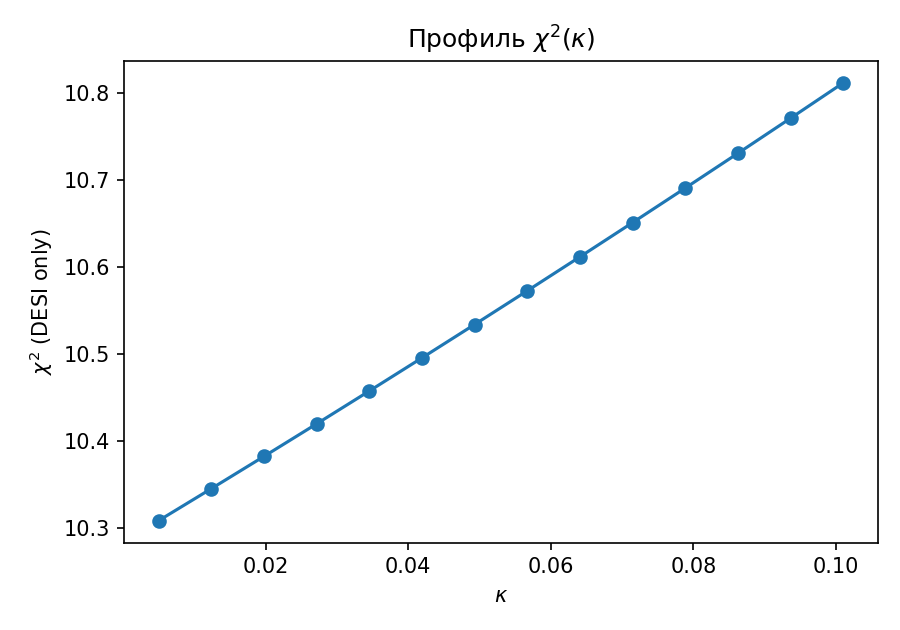
\includegraphics[width=0.65\textwidth]{profile_kappa.png}
\caption{The $\chi^2(\kappa)$ profile in the simplified model ($\beta=0$, $\alpha=0$, DESI only). It increases monotonically from $\chi^2=10.308$ ($\kappa=0.005$) to $\chi^2=10.811$ ($\kappa=0.101$); $\Delta\chi^2=0.53$ relative to the minimum, the level $\Delta\chi^2=1$ is not reached. The data do not constrain $\kappa$; the bound $\kappa\le0.101$ is perturbative.}
\label{fig:kappa}
\end{figure}

\section{Closure and Perturbation Stability}
The first closure is adiabatic, following from the accumulation dynamics itself. The sound speed as a thermodynamic response at fixed microphysics ($\lambda$ is a model parameter, not a state variable):
\[
c_s^2=\frac{\partial p}{\partial\rho}=w+\rho_x\frac{\partial w}{\partial\rho_x}=w+x\frac{dw}{dx}=w+\frac{\kappa x}{3},
\]
whence
\begin{equation}
c_s^2(\text{adiab})=-1-\frac{\kappa}{3}(1-2x)+\frac{\lambda(N)}{3}.
\label{eq:cs}
\end{equation}
The sign in front of the term $(\kappa/3)(1-2x)$ is negative; the derivation is confirmed: at the working point $c_s^2=-0.991$. In the entire allowed window $\kappa\le\lambda_0/(1-x_0)$ this quantity is negative: the upper estimate is $c_s^2\le-1+\lambda_0/3+\kappa_{\max}/3\approx-0.936<0$. An imaginary sound speed implies instability at small scales, and the adiabatic closure is excluded. Note: when the adiabatic sound speed is defined along the full background evolution (including the explicit dependence of $\lambda(N)$), an additional term $+\alpha\lambda(N)/[3(\lambda-\kappa(1-x))]$ appears; for small $\alpha$ it is negligible and does not change the conclusion.

The second closure is the standard one for effective dark energy theory: the declared sound speed $c_s^2=1$. This is not a consequence of the accumulation dynamics but an independent addition to the model, standard in working calculations. With this choice the dark energy sound horizon is comparable to the cosmological horizon (of order the particle horizon), perturbations at all observed scales smaller than the horizon are erased, and the influence of the medium on structure growth proceeds only through the background (Fig.~\ref{fig:wz}).

\begin{figure}[h]
\centering
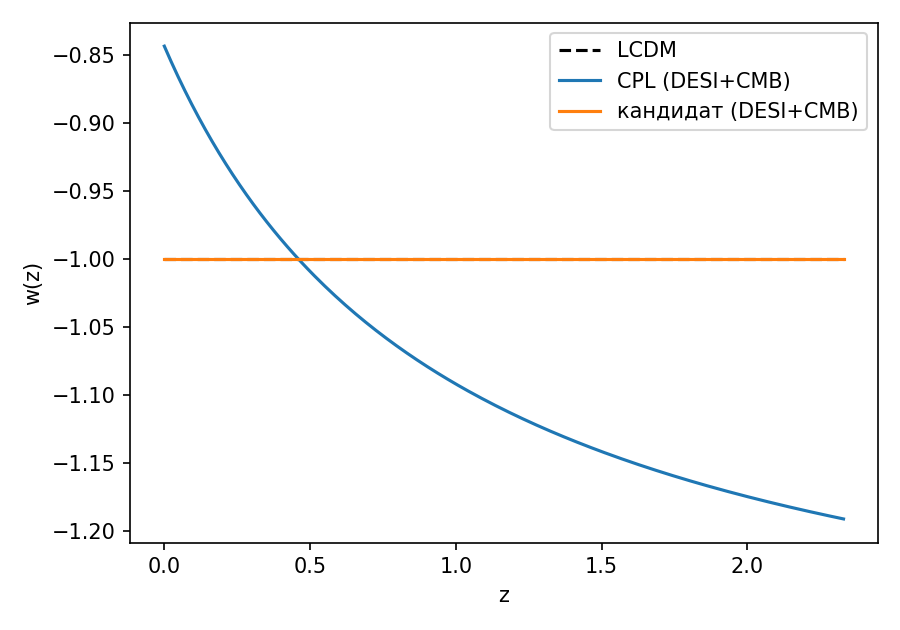
\includegraphics[width=0.65\textwidth]{wz_curves.png}
\caption{Equation of state $w(z)$: $\Lambda$CDM (dashed), CPL for DESI+CMB (solid), and the candidate (DESI+CMB). The candidate collapses to $\kappa=\lambda_0=0$, where it coincides with $\Lambda$CDM.}
\label{fig:wz}
\end{figure}

The perturbative bound is independent of the closure choice: the no-ghost condition $w>-1$ is a property of the background dynamics. Today it gives $\kappa\le\lambda_0/(1-x_0)=0.09/0.889\approx0.101$. The $\chi^2(\kappa)$ profile in the window $\kappa\le0.101$ is monotonic, $\Delta\chi^2=0.53<1$: the data do not constrain $\kappa$, and the bound remains perturbative. The statement that ``data and theory give the same bound'' is retracted; the data do not set a bound.

\section{Equation-of-State Ceiling at Finite $x$}
The ceiling $w\le-1+\lambda_0/3=-0.97$ is proven for arbitrary finite $x$ (see Eq.~\eqref{eq:w}): the term $\kappa_{\rm eff}(1-x)$ is non-negative for $\kappa_{\rm eff}\ge0$ and $x\in[0,1]$, and $\lambda(N)\le\lambda_0$ for $N\le0$. Equality is reached only in the double limit $\kappa\to0$ and $\lambda\to\lambda_0$; finite $x$ only pushes $w_0$ deeper into the phantom zone. A numerical check over all scan points confirms the ceiling.

\section{Structure Growth}
The growth equation is solved for both models with their background histories; comparison is made with the $f\sigma_8$ compilation (11 points from $z=0$ to $z\approx0.9$). Results: $\chi^2=14.28$ for both models; the difference between the growth curves is $0.024\,\%$ at all redshifts; even a coupling of $0.35$ gives only $0.27\,\%$. The fitted normalizations are $\sigma_8=0.8717$ ($\Lambda$CDM) and $0.8719$ (model). The shift in normalization is a known systematic of redshift-space distortion measurements, common to all cosmologies, identical for both models, and does not affect the conclusion of indistinguishability.

The model is falsifiable, but distinguishing it from $\Lambda$CDM ($\Delta w_0=0.0063$) requires $\sigma(w_0)\le0.002$, i.e.\ a 25--70-fold improvement in precision, or an increase in data volume by hundreds to thousands of times. Realistic test channels are fourth-generation data and the shape of $w(z)$ at low redshifts.

\section{Attractor and Predictions}
The roots of the accumulation equation are $x=0$ and $x^*=1-\lambda/\kappa$, with $x^*$ stable. On the attractor $w\to-1$ exactly; the ceiling of the mechanism completes itself: the future is pure de Sitter (numerically: approaches $-1.0000$). If $\kappa<\lambda_0$, dark energy slowly dissolves; both regimes are healthy, with no big rip.

Falsification criteria: (i) a significantly strengthening phantom behavior $w_0<-1.05$ at small coupling; (ii) a reversal of expansion to contraction; (iii) compatibility with the DESI anomaly at the level of the full shape of $w(z)$, not the CPL projection.

\section{Conceptual Part}

\subsection{Arrow of Time and the Minus Sign}
The minus sign is a property of density and pressure (negative dark energy pressure, the minus in front of the decay term), not the direction of time. The model equations are not invariant under $N\to-N$: under $N\to-N$ the decay terms turn into growth terms; the direction is set by the structure of the dynamics. Irreversibility of events at the fundamental level is an initial postulate from which informational time is generated; the cosmological model accepts it and tests it for consistency rather than deriving it: background trajectories are reconstructible in both directions, and this is mathematics, not a defect. Testing the postulate lies at the level of microphysics.

\subsection{Observer's Window and Records Beyond the Horizon}
Three limits of the window. The technical one is instrument sensitivity; it recedes with time. The light cone: every photon is a trace of a past event, the more distant the further the source; the observed slowing of distant flashes is a measurable quantity, and the density of events in the past was higher. The particle horizon has a radius of about 46 billion light years; events beyond it will never leave records; the window is practically closed. The only legitimate access to the beyond is the statistics of early-Universe imprints: superhorizon perturbations frozen in during inflation are read off from the distribution of CMB anisotropies; individual anomalies remain at the level of hints.

\subsection{Cyclicity}
The model does not carry reverse flow: it would require invariance of the equations under reversal of the count and decreasing entropy; the first is violated by the structure, the second is outside the competence of cosmology. Cyclic constructions (bounce in quantum geometry, conformal cycles) are a living program with a common wound: a cycle must dispose of entropy somewhere. Contraction would require a change of sign of dark energy; the model in the allowed window does not permit this and answers: eternal acceleration, no reversal in the equations.

\section{Conclusions}
\begin{enumerate}
\item \textbf{The accumulation model does not explain the DESI anomaly and does not require non-zero parameters.} In both fits (DESI only and DESI+CMB) the full model $(\kappa,\beta,\lambda_0,\alpha)$ collapses to $\kappa=\lambda_0=0$, where it is identical to $\Lambda$CDM: $\beta\to0.004$ and $0.0003$, $\alpha\to0$, $\Delta\chi^2\approx0.000$. The matter channel and the decay are not felt; the simplification $\alpha=\beta=0$ as the working limit of the model is justified. The CPL anomaly in BAO alone is weak ($\Delta\chi^2=-4.67$); with the DESI prior and the $\theta_*$ calibration, $-4.09$; with the CHW prior, $-3.50$. The previous value $-9.87$ was an artifact of the hand-built table ($\sigma(\text{LRG2 }D_H)$ underestimated by a factor of two) and is annulled.

\item \textbf{The matter channel is excluded by three independent methods:} parameter scan (60 starts per point), big bang nucleosynthesis (bound $2\times10^{-28}$), and perturbative instability. The ghost threshold follows from the full equation $\kappa_{\rm eff}(1-x)=\lambda(N)$: at the working coupling any $\beta>0$ gives $w<-1$ from $z_{\rm crit}\le2.5$, and for $\beta\ge0.1$ already at $z\approx0$. Close to the perturbative ceiling $w>-1$ any non-zero $\beta$ is immediately unphysical. In the fit the channel $\beta$ is not activated ($\beta\to0$), consistent with these constraints.

\item \textbf{The perturbative bound $\kappa\le0.101$ is a quantitative result independent of the closure choice.} It follows from the no-ghost condition $w>-1$ (a property of the background dynamics) and uses neither data nor the perturbation closure. The $\chi^2(\kappa)$ profile in the window $\kappa\le0.101$ is monotonic, $\Delta\chi^2=0.53<1$: the data do not constrain $\kappa$, and the bound remains perturbative. The statement that ``data and theory give the same bound'' is retracted; the data do not set a bound.

\item \textbf{The ceiling $w\le-0.97$ is global;} the thawing zone is unreachable at any finite $x$.

\item \textbf{Within the stable window the model is indistinguishable from $\Lambda$CDM in structure growth ($0.024\,\%$)} and predicts an exact de Sitter attractor; a viable candidate with explicit falsification criteria.
\end{enumerate}

\section{Caveats}
\begin{enumerate}
\item The smooth dark energy approximation at $c_s^2=1$ is a standard approximation of working codes, stated explicitly.
\item The shift $\sigma_8=0.87$ is a systematic of redshift-space distortion measurements, common to all models; the difference in normalizations between $\Lambda$CDM and the model is $0.0002$.
\item The conceptual section (9) does not enter the quantitative results; its testable consequences lie in the microscopic part of the program.
\item Distinguishability in the background lies beyond the horizon of current-generation programs.
\item The prior $(\theta_*,\omega_b,\omega_{bc})$ is taken from Appendix A of DESI DR2 Results II (CamSpec); $\mathrm{TH\_CAL}=1.0026$ calibrates $\theta_*$ against the fiducial. The residual discrepancy with the official $\Delta\chi^2=-8.5$ is due to the simplified early-Universe physics. The Chen--Huang--Wang (2019) prior is used as a systematic check: $\Delta\chi^2=-3.50$.
\item DESI DR2 data are loaded from the official release files (mean and cov); the hand-built table used in draft calculations contained errors ($\sigma(\text{LRG2 }D_H)$ underestimated by a factor of two; three correlations shifted) and is annulled.
\end{enumerate}

\appendix
\section{Compressed DESI DR2 Prior (Appendix A, CamSpec)}
\label{app:priors}
\[
\mu=(0.0104110,\ 0.02223,\ 0.14208),\qquad
\mathbf{C}=10^{-9}\times\begin{pmatrix}
0.006621 & 0.12444 & -1.1929\\
0.12444 & 21.344 & -94.001\\
-1.1929 & -94.001 & 1488.4
\end{pmatrix}.
\]
Calibration: $\mathrm{TH\_CAL}=0.0104110/\theta_*^{\rm th}(h=0.6766,\omega_b=0.02223,\omega_{bc}=0.14208)=1.0026$.
Systematic check (Chen, Huang, Wang 2019): $R=1.7493\pm0.0046$; $\ell_A=301.462\pm0.090$; $\omega_b=0.02239\pm0.00015$; $\rho(R,\ell_A)=0.47$, $\rho(R,\omega_b)=-0.66$, $\rho(\ell_A,\omega_b)=-0.34$.

\begin{thebibliography}{99}
\bibitem{desi_dr2} DESI Collaboration (Abdul-Karim, M., et al.), \textit{DESI DR2 Results II: Measurements of Baryon Acoustic Oscillations and Cosmological Constraints}, arXiv:2503.14738 [astro-ph.CO] (2025).
\bibitem{desi_lya} DESI Collaboration, \textit{DESI DR2 Results I: Lyman-$\alpha$ forest BAO}, arXiv:2503.14739 [astro-ph.CO] (2025).
\bibitem{planck2018} Planck Collaboration (Aghanim, N., et al.), \textit{Planck 2018 results. VI. Cosmological parameters}, Astron.\ Astrophys.\ \textbf{641}, A6 (2020), arXiv:1807.06209.
\bibitem{chen2019} Chen, L., Huang, Q.-G., Wang, K., \textit{Distance Priors from Planck Final Release}, J.\ Cosmol.\ Astropart.\ Phys.\ \textbf{02}, 028 (2019), arXiv:1808.05725.
\bibitem{copeland2006} Copeland, E.~J., Sami, M., Tsujikawa, S., \textit{Dynamics of dark energy}, Int.\ J.\ Mod.\ Phys.\ D \textbf{15}, 1753 (2006), arXiv:hep-th/0603057.
\bibitem{penrose2010} Penrose, R., \textit{Cycles of Time: An Extraordinary New View of the Universe}, Bodley Head (2010).
\bibitem{fsigma8} Sánchez, A.~G., et al., \textit{The clustering of galaxies in the completed SDSS-IV eBOSS survey: cosmological constraints}, Mon.\ Not.\ R.\ Astron.\ Soc.\ \textbf{500}, 736 (2021), arXiv:2007.08993.
\end{thebibliography}

\end{document}